\documentclass[letterpaper,12pt]{report}
\usepackage[utf8]{inputenc}
\usepackage[english, russian]{babel}
\usepackage[backend=biber, style=ieee, sorting=none]{biblatex} % TODO: sort citations by their appearance and also edit autogenerated .bib
\usepackage{hyperref}
\usepackage{xltabular} % TODO: compare with tabular, longtable, xtabular, xtab, tablearray, xltabular, ltablex, tabularx
\usepackage{graphicx} % TODO: what is this package for? 
\usepackage{amsmath} % TODO: check if it is really affect on setcounter numbering of sections

\addbibresource{references.bib}

\hypersetup{
    colorlinks=true,
    linkcolor=blue,
    citecolor=blue,
    filecolor=blue,
    urlcolor=blue
}

\graphicspath{{figures/}}

\begin{document}

\title{Assignment 2: Advanced Computer Networks Security}
\author{Tendikov N. M. \\ [0.5ex]
        SSE-2401 \\ [0.5ex]
        Astana IT University}
\date{\today}
\maketitle

\section{Theory}
1. STRIDE - a model/framework for threat modeling and risk management made by Microsoft. Its alternatives: PASTA (Process for Attack Simulations and Threat Analysis), DREAD, CIA, CIADIE, LINDDUN, PLOT4ai, etc.

% TODO: change to 25, 25, 50, tabural inside table (table vs table environment)
\begin{xltabular}{\linewidth}{|X|X|X|}
\hline
\multicolumn{1}{|c|}{\textbf{Type}} & \multicolumn{1}{c|}{\textbf{Mitigation/Control}} & \multicolumn{1}{c|}{\textbf{Description}} \\
\hline
Spoofing & Authentication & Threat action aimed at accessing and use of another user's credentials, such as username and password. \\
\hline
Tampering & Integrity & Threat action intending to maliciously change or modify persistent data, such as records in a database, and the alteration of data in transit between two computers over an open network, such as the Internet. \\
\hline
Repudiation & Non-Repudiation & Threat action aimed at performing prohibited operations in a system that lacks the ability to trace the operations. \\
\hline
Information disclosure & Confidentiality & Threat action intending to read a file that one was not granted access to, or to read data in transit. \\
\hline
Denial of service & Availability & Threat action attempting to deny access to valid users, such as by making a web server temporarily unavailable or unusable. \\
\hline
Elevation of privilege & Authorization & Threat action intending to gain privileged access to resources in order to gain unauthorized access to information or to compromise a system. \\
\hline
% TODO: here оступ нужен от описания
\caption{STRIDE categories of threats and their security mitigations/controls}
\end{xltabular}

2. DFD (Data Flow Diagram) - a diagram notation for designing business process, but well applied in threat modeling. Generally, it provides a high-level understanding of the available resources and the direction of data at multiple levels of detailization (from 0 to multi-level, similar to C4 model). The main elements of DFD: entities / actors, processes, data stores, and data flows. There are various tools (specialized and general) that are used for DFD visualization: Microsoft Threat Modeling Tool, OWASP Threat Dragon, draw.io, pseudocode, etc. Possible alternatives: flowchart, bpmn, transcation flow, activity diagram, and so on.

\section{Practice}

\subsection{System scope and overview}
We have examined the PyPI platform, which hosts a large number of different Python packages. It is owned by the Python Software Foundation (PSF), but operates under a free and open model, where any user may use the package manager or other mechanisms to upload, download, and publish packages in the form of source or build distributions. Similar systems and policies are followed by other software repositories and ecosystems, such as Maven Central, NPM, Crates.io, and many others.

The analysis was divided into several parts, focusing on specific features rather than the entire product at once (logical vs physical DFD). Certain elements and details were omitted, and some components were grouped in a manner that may appear ambiguous, due to underlying assumptions and presumptions, as not all architectural aspects of the system are fully known to us. Since it is not always possible to apply a white-box approach, we also have to work with black-box systems, where the specific technologies remain unidentified. In such cases, only a high-level representation is available, emphasizing specifications and general characteristics rather than implementations and specific details. Extensive details demands additional time and resources (and is more appropriate for reverse engineering), whereas in threat modeling the primary objective is to establish a model that is sufficiently representative.

In future, instead of just happy path, we need more complex conditionals and error handling for specific cases (infrastructure error like database problem or out of memory error).

\subsection{Data flow and activity diagrams}

We prepared a DFD legend with all necessary elements for drawing process as represented in figure 1. Also, constructed level 0 DFD as shown in figure 2.
\begin{figure}[htpb!]
    \centering
    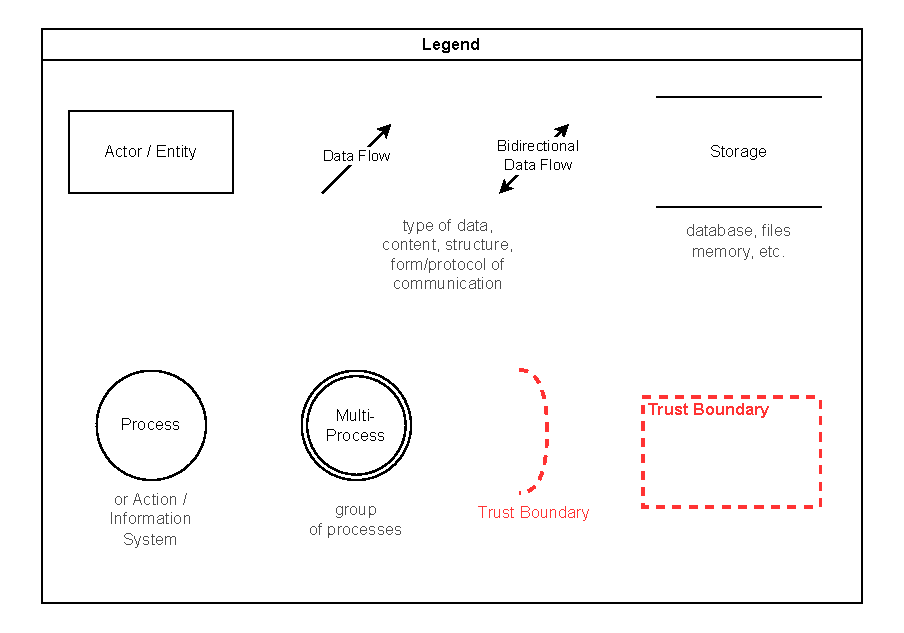
\includegraphics[width=0.5\textwidth]{figure_1}
    \caption{Legend of DFD}
    \label{fig:figure1}
\end{figure}

\begin{figure}[htpb!]
    \centering
    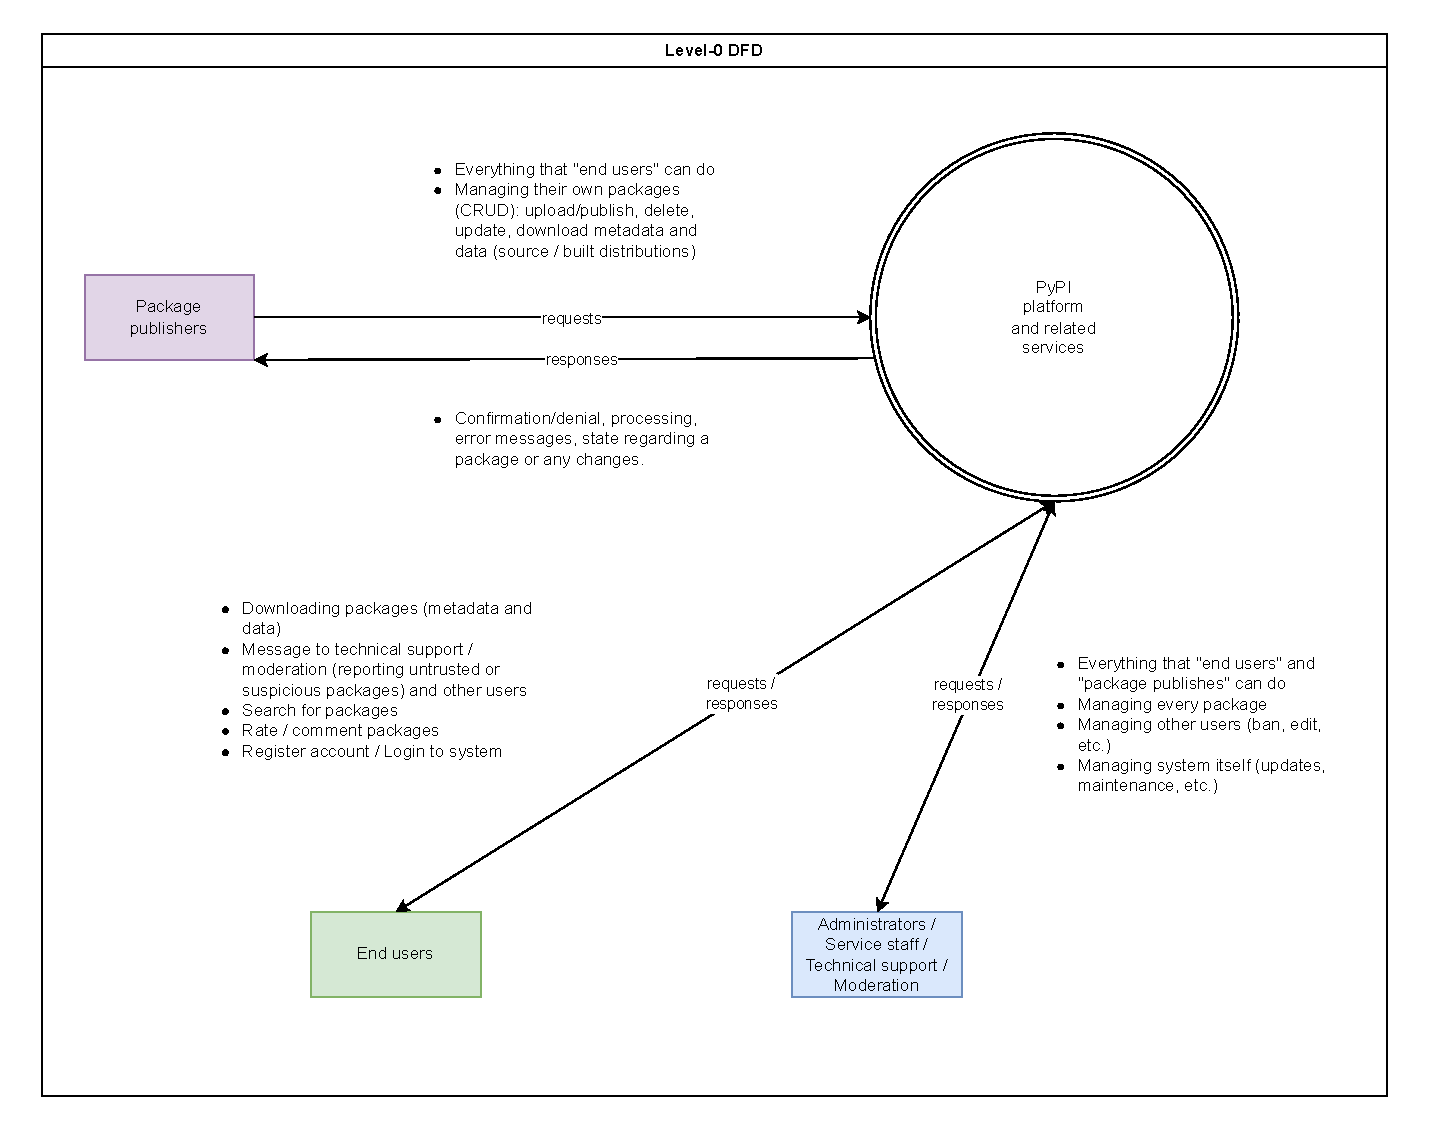
\includegraphics[width=1\textwidth]{figure_2}
    \caption[Level-0 DFD]
    \label{fig:figure2}
\end{figure}

Based on level 0, we delved into the details and produced Level-1 DFD subdiagrams and activity diagrams for specific features, including descriptions of the client–server model, communication protocols, and related interactions. We consciously decided to omit aspects concerning connectivity to the internet (e.g., Internet service providers and intermediary network components), as those elements fall outside the scope of this analysis.
Interaction interfaces with the platform and general logical DFD:
\begin{itemize}
    \item Registered domain name ("pypi.org") is being resolved by some DNS hosting service (e.g. Cloudflare).
    \item Firewall limiting activity and filters traffic.
    \item Mirroring and reverse proxy garantees lower load за счет перераспределения нагрузки на альтернативные источники (geographically distributed network, взаивисмости от локального расположения или доступности сервера, multiple instances of PYPI that replicates data).
    \item Different types of sensitivity (confidential / internal / public), system boundaries, trusted/untrusted zones.
    \item Cloud hosting service / on-premises.
    \item RPC/GRPC/REST internal communcation between microservices.
    \item Не рассмотрели: web admin panel, register / login to platform (authentication / authorization), payment system, and so on...
\end{itemize}

% TODO: force images to be grouped or on same page
\begin{figure}[htpb!]
    \centering
    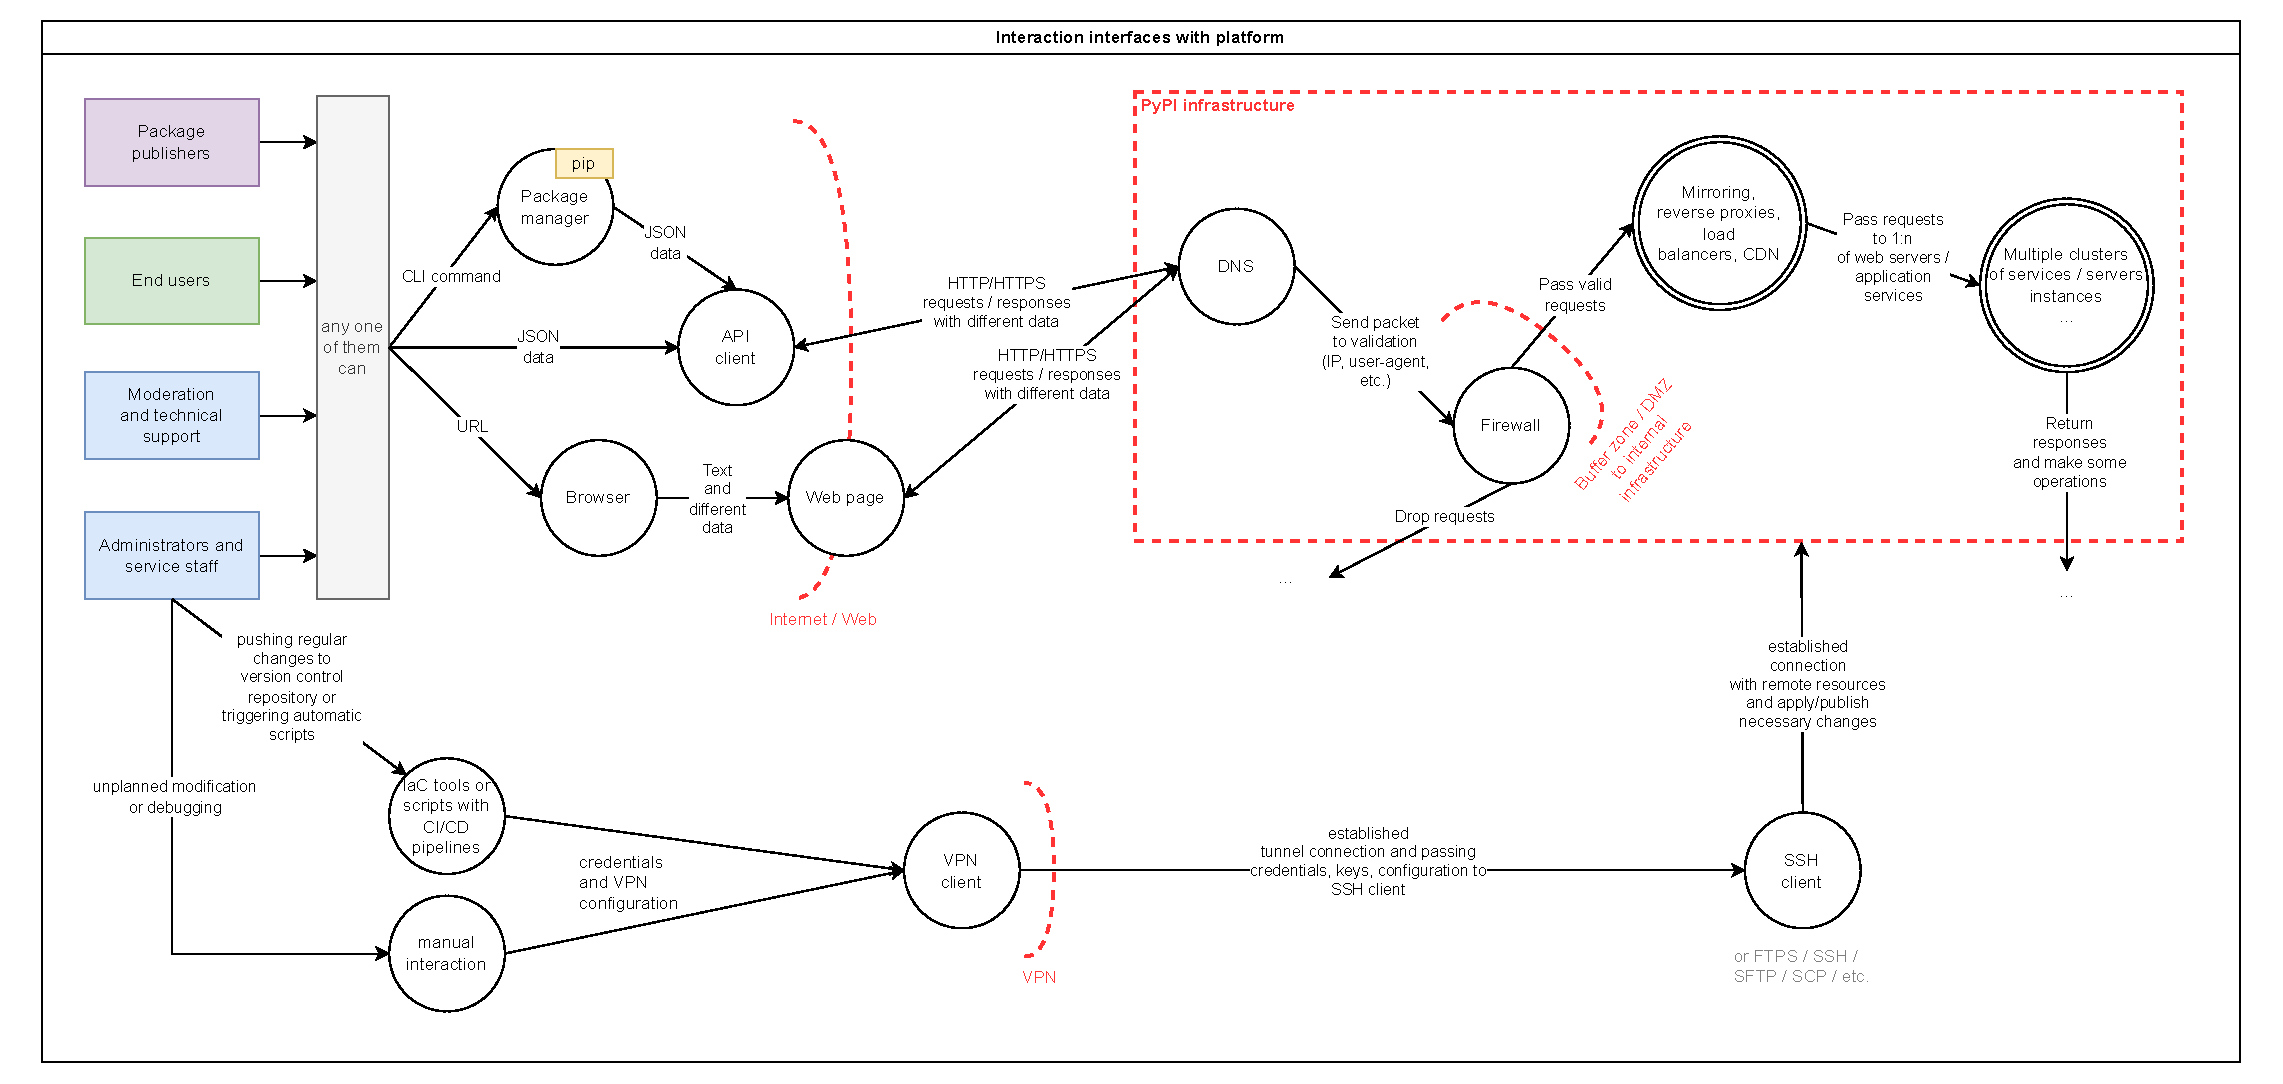
\includegraphics[width=1\textwidth]{figure_3}
    \caption[Interaction interfaces with the platform]
    \label{fig:figure3}
\end{figure}

\begin{figure}[htpb!]
    \centering
    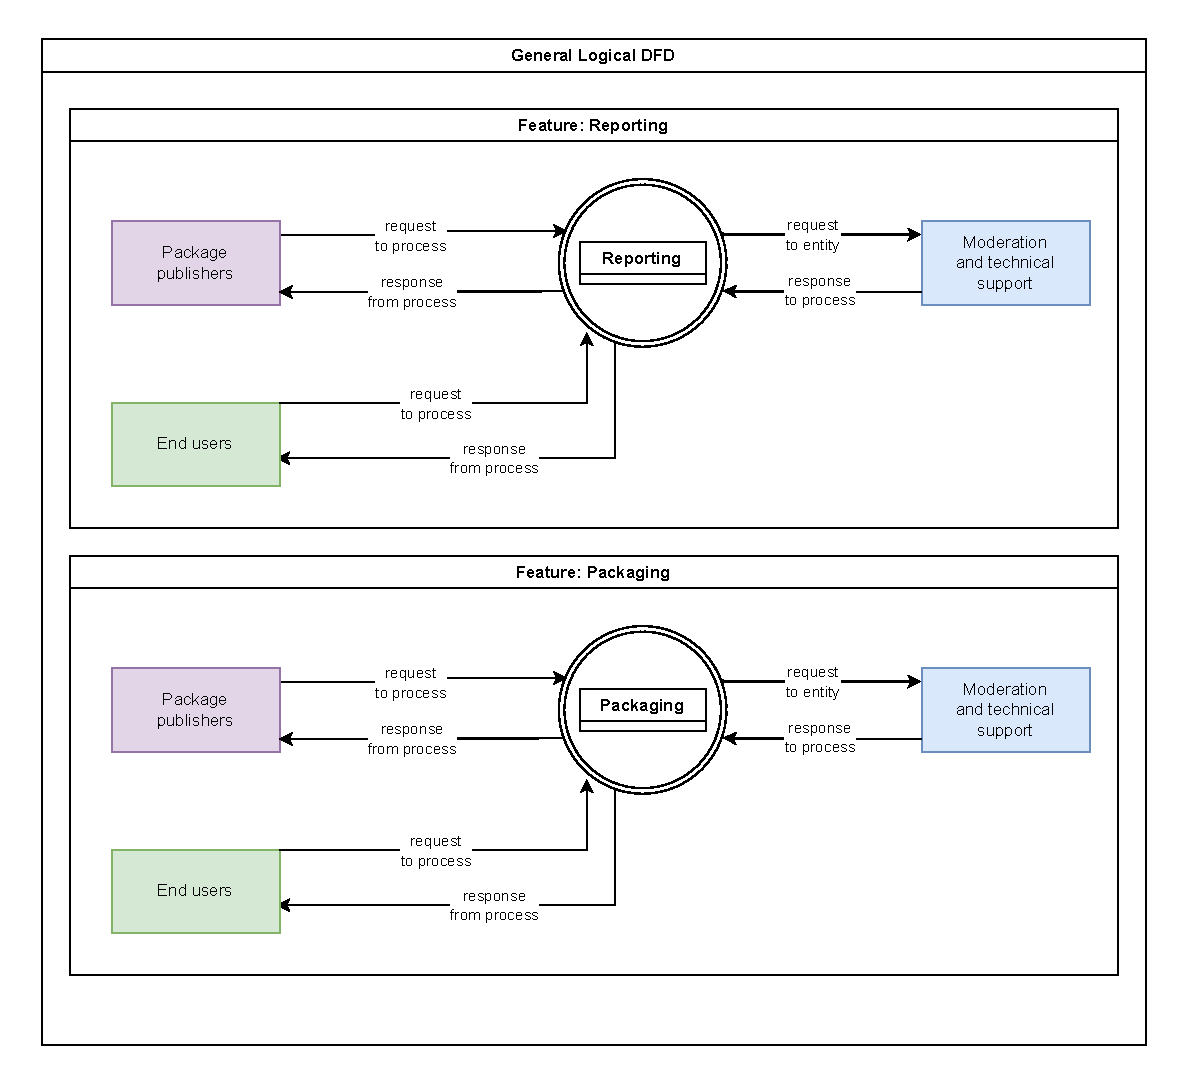
\includegraphics[width=0.7\textwidth]{figure_4}
    \caption[General logical DFD]
    \label{fig:figure4}
\end{figure}

\begin{figure}[htpb!]
    \centering
    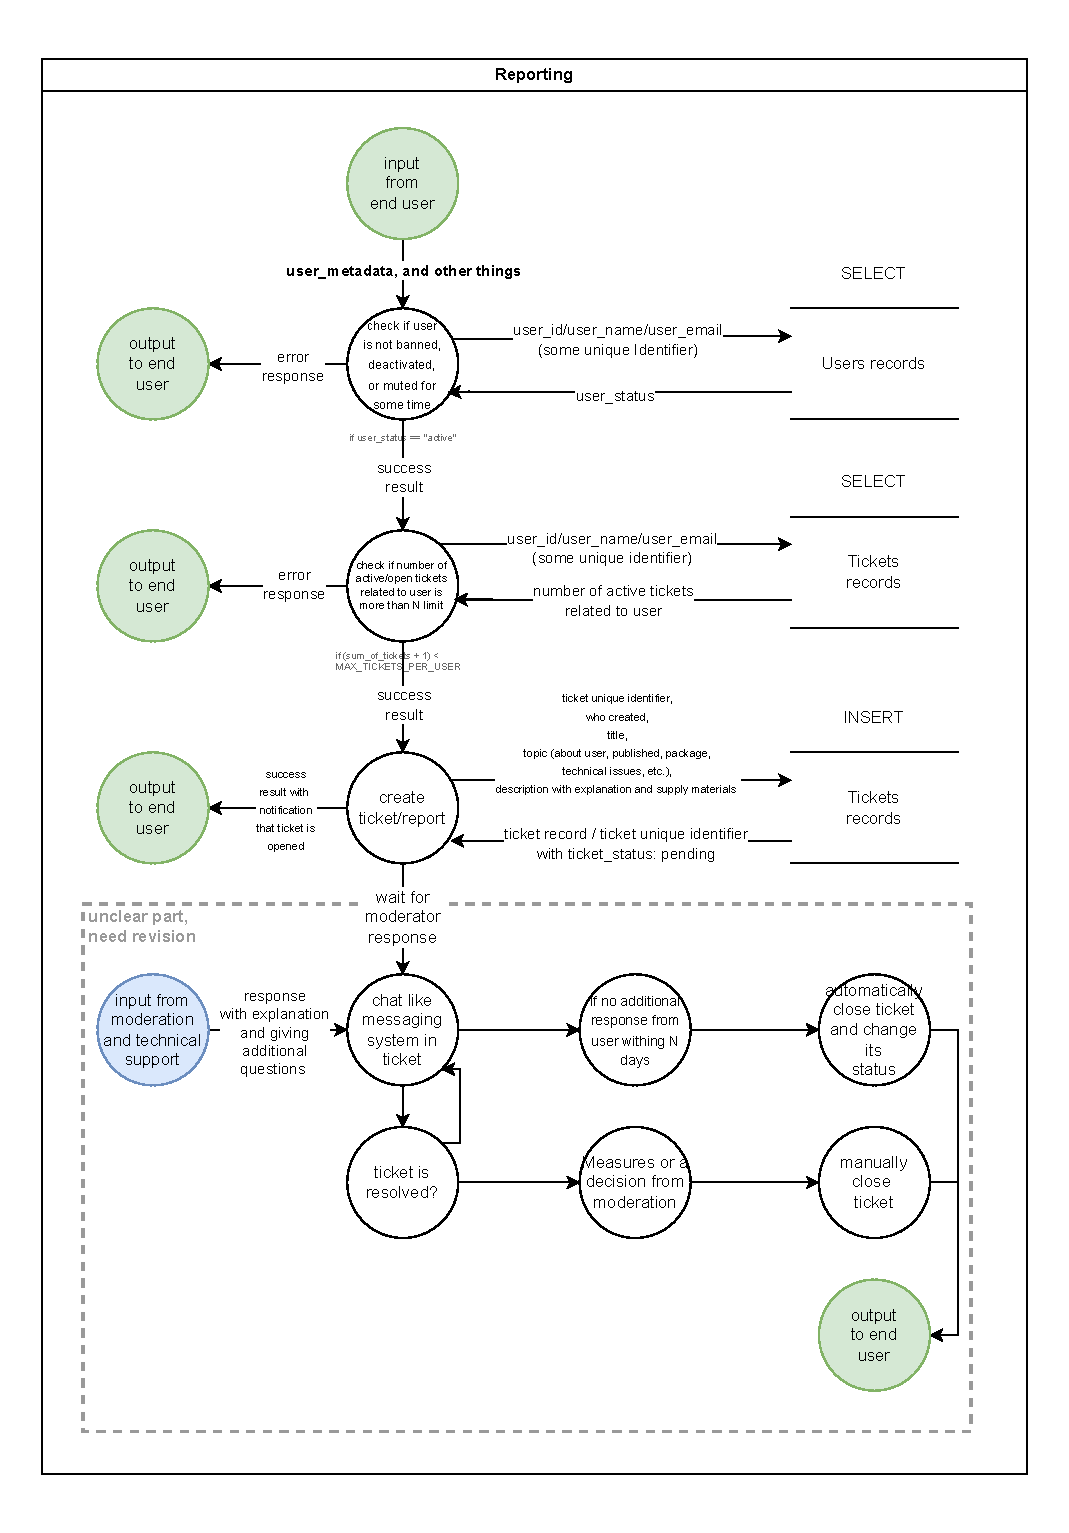
\includegraphics[width=1\textwidth]{figure_5}
    \caption[Feature: Reporting]
    \label{fig:figure5}
\end{figure}

\begin{figure}[htpb!]
    \centering
    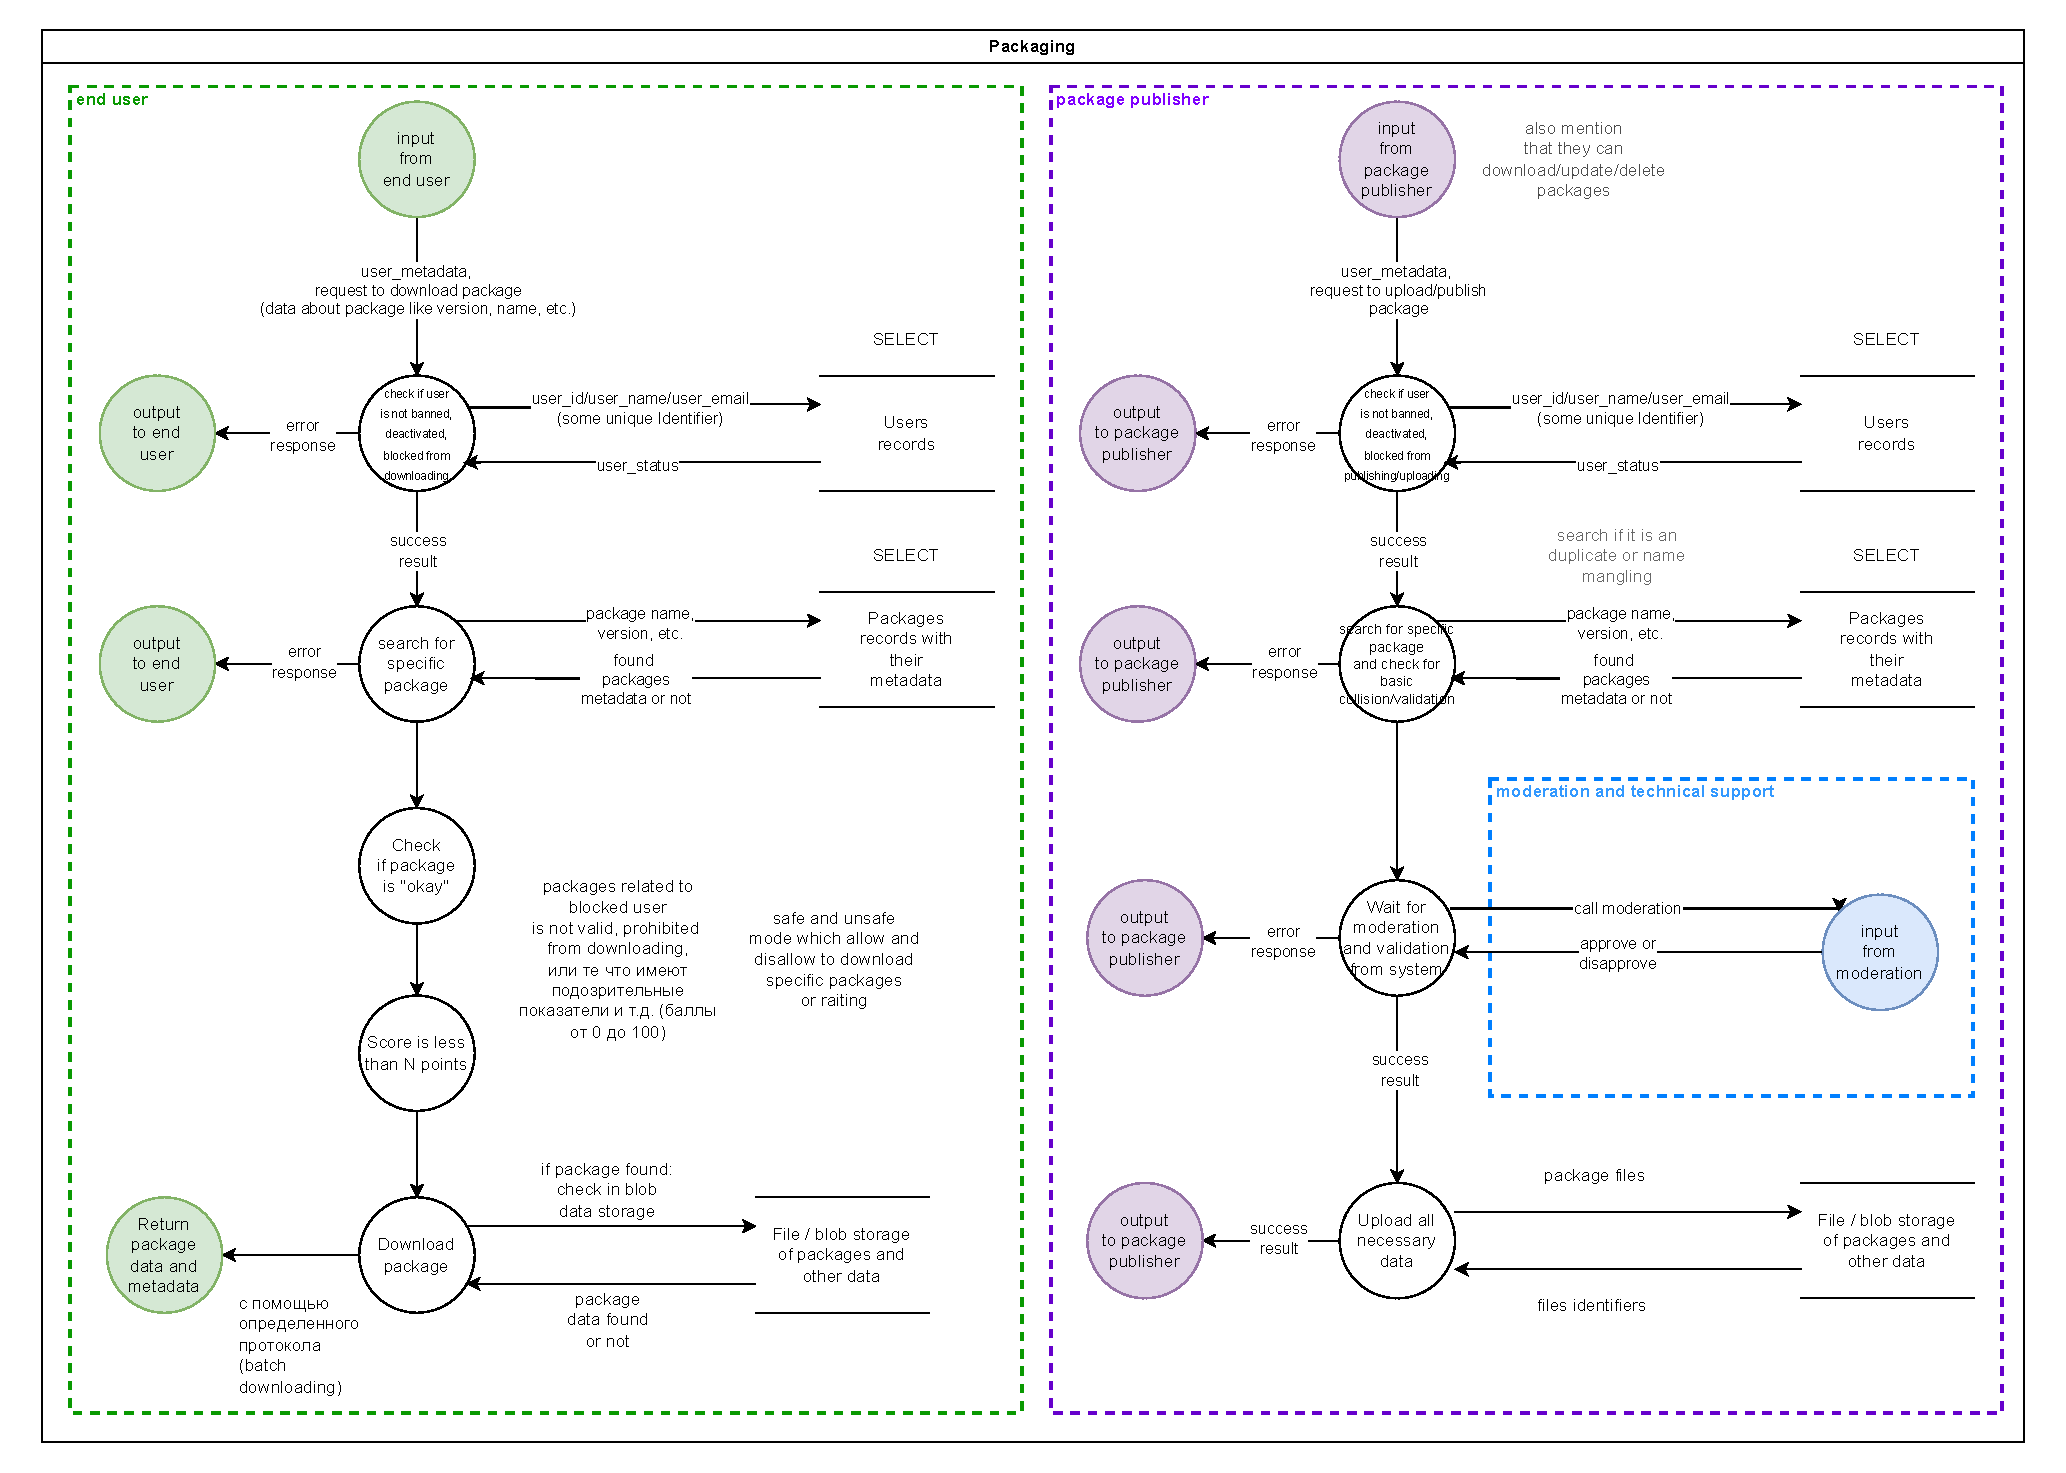
\includegraphics[width=1\textwidth]{figure_6}
    \caption[Feature: Packaging]
    \label{fig:figure6}
\end{figure}
\newpage

\subsection{STRIDE analysis}
% TODO for all DFD elements (process, flow, data store, entity)
% add likelihood (H/M/L) and impact (H/M/L), short description, potential attack vectors / prerequisites,

\begin{xltabular}{\textwidth}{|X|X|X|X|X|}
\hline
\textbf{STRIDE Category} & \textbf{Threat Description} & \textbf{Attack Vector} & \textbf{Likelihood} & \textbf{Impact} \\
Spoofing & Typosquatting / malicious packages impersonating popular projects & Publish similarly-named packages to trick users (typosquatting). & Medium & High \\
\hline
Spoofing & Account takeover of a legitimate maintainer & Phishing, credential stuffing, SSO/email compromise to gain push privileges. & High & High \\
\hline
Tampering & Malicious modification of package artifacts (binaries/source) & Compromise of CI/CD pipeline, upload of backdoored builds, or artifact replacement at rest. & Medium & High \\
\hline
Tampering & Metadata tampering (hashes, versioning) & Unauthorized modification of package metadata or index entries to point to malicious artifacts. & Medium & Medium \\
\hline
Repudiation & Denial of malicious release or action by a maintainer & Use of compromised or shared keys; absence of cryptographic non-repudiation for uploads. & Low--Medium & Medium \\
\hline
Repudiation & Deletion/alteration of audit/moderation logs & Insider action or compromise of logging backend to remove evidence. & Low & High \\
\hline
Information Disclosure & Accidental leakage of secrets inside packages & Developers accidentally commit API keys, credentials, or secrets in source distributions. & High & High \\
\hline
Information Disclosure & Repository infrastructure/data breach & Compromise of backend servers or storage exposing user data and unpublished artifacts. & Medium & High \\
\hline
Denial of Service & Download / upload floods and CDN exhaustion & High-volume request floods, abuse of upload API, or large artifact spam. & Medium & High \\
\hline
Denial of Service & Package disappearance / dependency disruptions & Mass yanking or deletion (or corruption) of popular packages causing downstream breakage. & Low--Medium & Medium \\
\hline
Elevation of Privilege & Unauthorized promotion to project owner / moderator & Exploitation of RBAC misconfigurations, abused account recovery, or social engineering of staff. & Medium & High \\
\hline
Elevation of Privilege & Compromise of platform service accounts or orchestration plane & Stolen service/API keys, leaked credentials, or vulnerable management interfaces enabling admin actions. & Medium & High \\
\hline
\caption{STRIDE analysis for a PyPI-like repository}
\end{xltabular}

\subsection{Attack scenario}
We modeled some attack lifecycles, attack surface / tree with details, and kill chain scenaries.

\begin{figure}[htpb!]
    \centering
    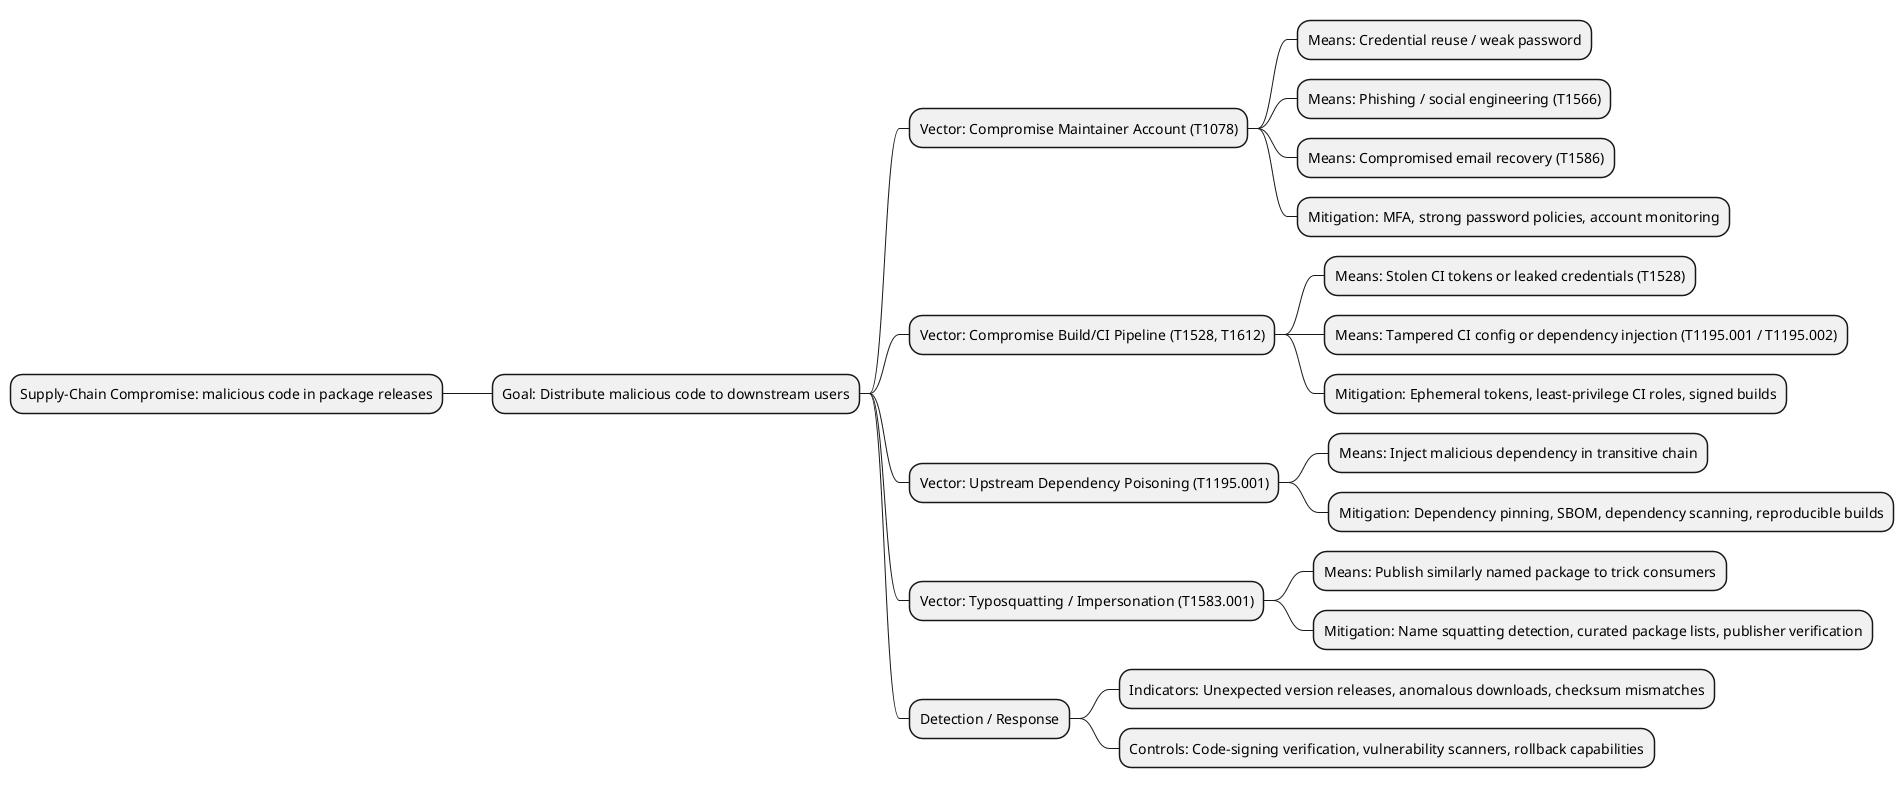
\includegraphics[width=1\textwidth]{figure_7}
    \caption[Attack scenario 1]
    \label{fig:figure7}
\end{figure}

\begin{figure}[htpb!]
    \centering
    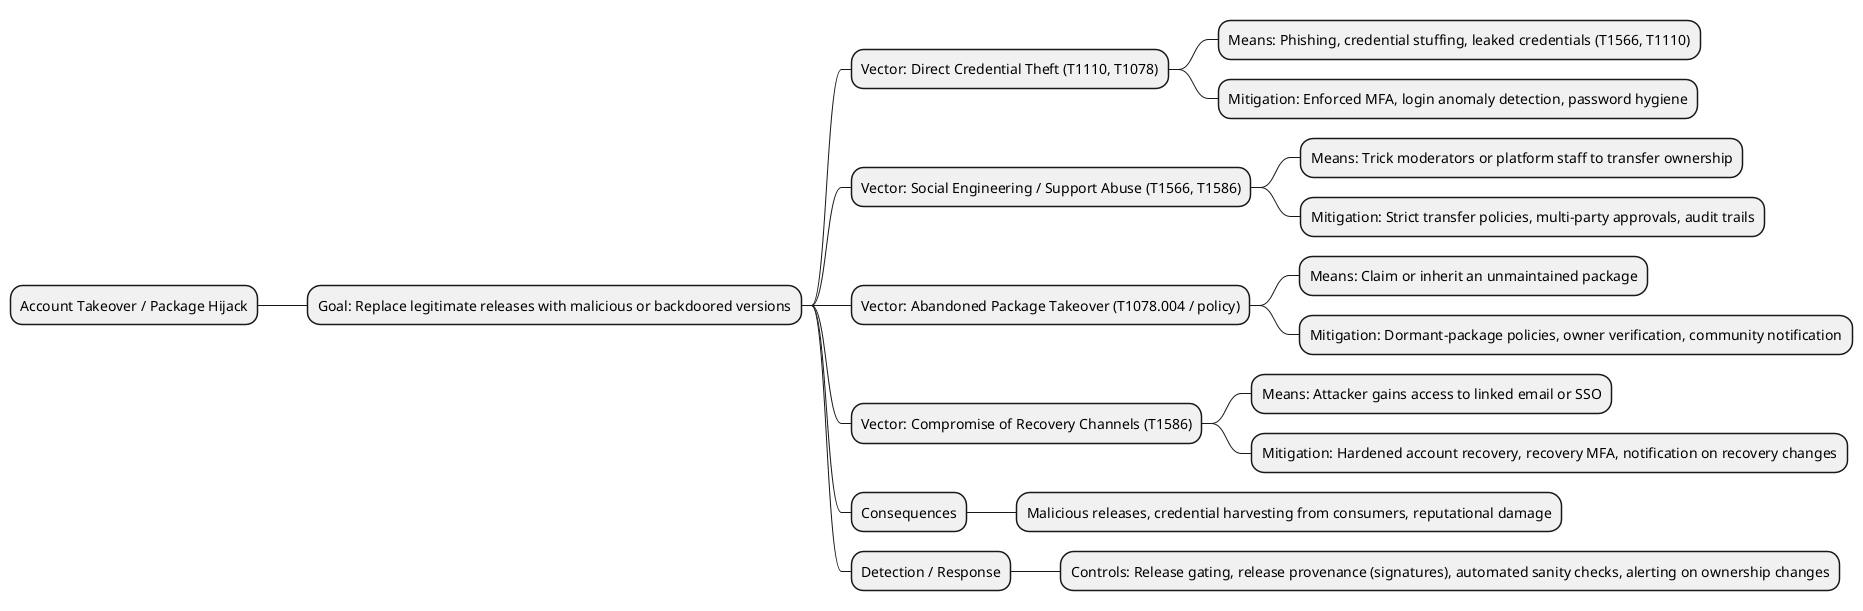
\includegraphics[width=1\textwidth]{figure_8}
    \caption[Attack scenario 2]
    \label{fig:figure8}
\end{figure}

\begin{figure}[htpb!]
    \centering
    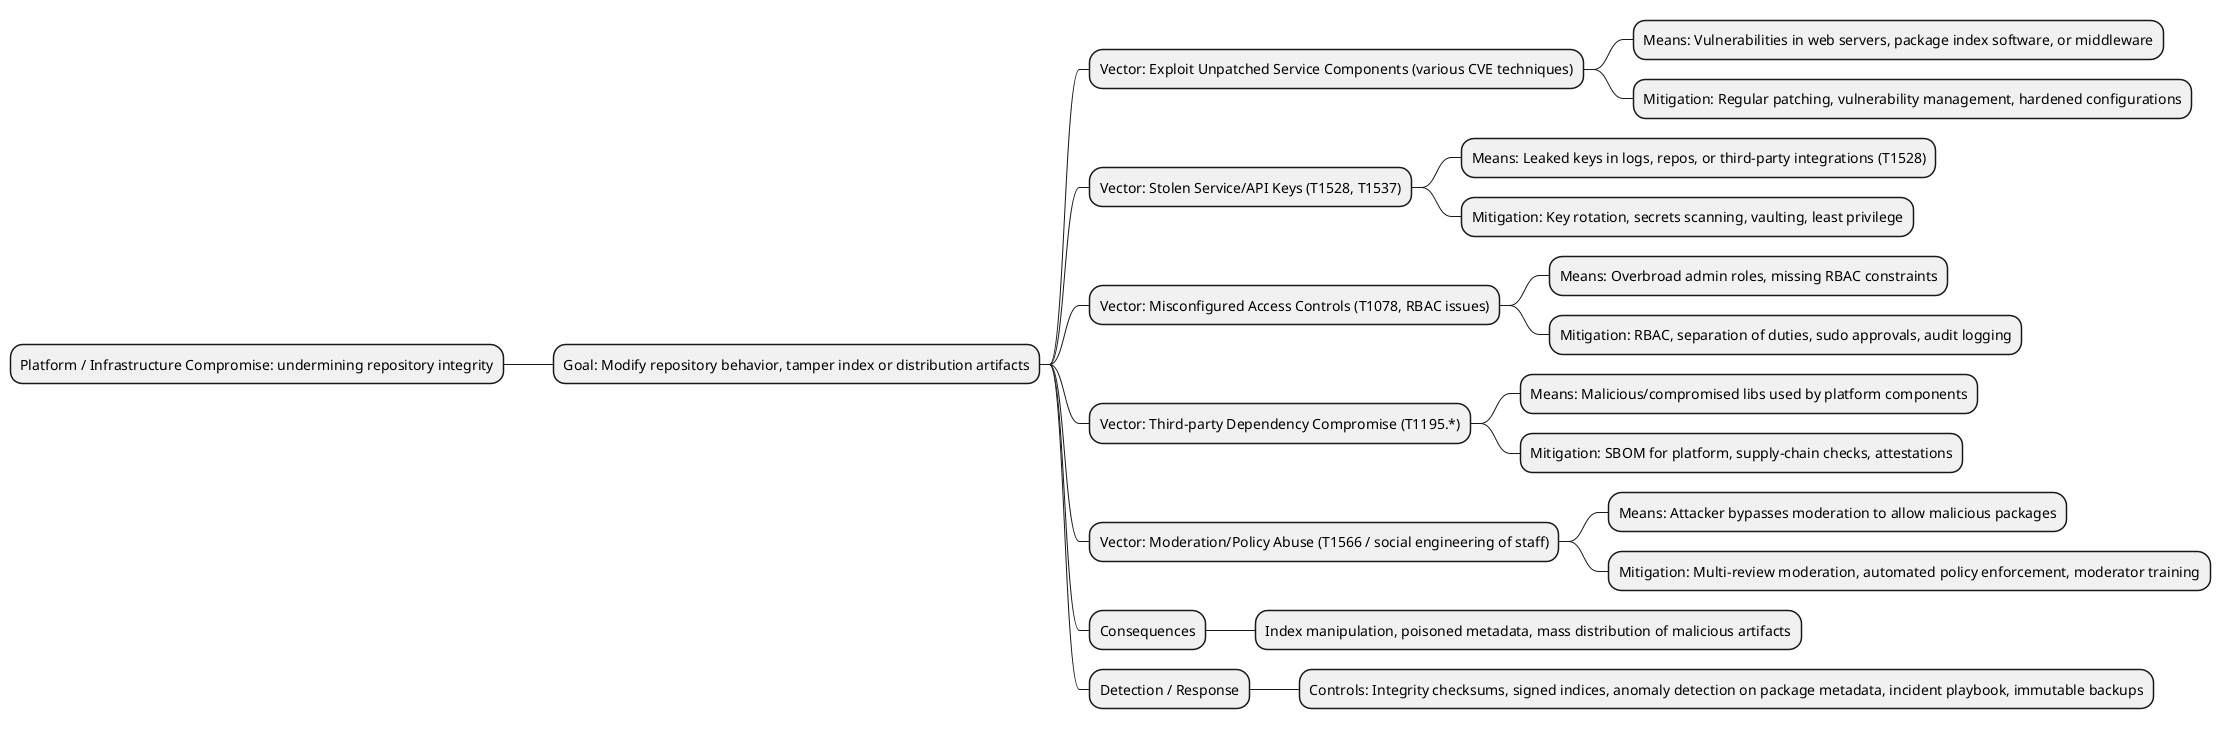
\includegraphics[width=1\textwidth]{figure_9}
    \caption[Attack scenario 3]
    \label{fig:figure9}
\end{figure}

\newpage

\subsection{Risk assessment, mitigation and counter measures}
% countermeasures, Assess each scenario’s risk using a simple matrix: Risk = Likelihood × Impact (H/M/L).
% Propose technical controls (MFA, WAF, segmentation, TLS 1.3, patches) and organizational measures (policies, awareness training, logging).
% For each measure, explain (justifications): expected risk reduction, implementation effort, and validation metrics.
% Risk assessment matrix, Recommendations for monitoring and detection.
% Countermeasures and implementation plan.

This section evaluates each STRIDE category threat, assigns risk severity based on the 
matrix (Risk = Likelihood $\times$ Impact), and proposes mitigation strategies.  
Technical, organizational, and monitoring controls are combined for defense-in-depth.

\subsubsection*{Spoofing}

\textbf{Typosquatting / malicious packages.}  
Risk: Medium--High (2 $\times$ 3 = 6).  
\emph{Mitigation:} Introduce package name similarity detection, automated blocking of 
lookalike names, and mandatory maintainer verification.  
\emph{Justification:} Prevents attacker-driven namespace abuse. Medium effort (policy and 
automation). Validation via quarterly red-team tests and false-positive review metrics.  

\textbf{Account takeover of legitimate maintainers.}  
Risk: Critical (3 $\times$ 3 = 9).  
\emph{Mitigation:} Enforce MFA, strong SSO policies, credential rotation, and anomaly-based 
login monitoring.  
\emph{Justification:} Eliminates single-factor credential compromise. High impact reduction, 
medium operational effort. Validation via access log audits and simulated phishing campaigns.  

\subsubsection*{Tampering}

\textbf{Malicious modification of package artifacts.}  
Risk: Medium--High (2 $\times$ 3 = 6).  
\emph{Mitigation:} Use reproducible builds, signed artifacts, and secured CI/CD with 
hardware-backed signing keys.  
\emph{Justification:} Ensures build integrity. Requires DevSecOps investment. Validation 
through artifact signature verification and pipeline penetration tests.  

\textbf{Metadata tampering.}  
Risk: Medium (2 $\times$ 2 = 4).  
\emph{Mitigation:} Immutable version indexes, TLS~1.3 everywhere, integrity checks 
with transparency logs.  
\emph{Justification:} Preserves metadata trustworthiness. Low--medium effort. Validation 
via automated integrity scans.  

\subsubsection*{Repudiation}

\textbf{Maintainer denial of malicious releases.}  
Risk: Medium (2 $\times$ 2 = 4).  
\emph{Mitigation:} Enforce signed uploads, publish cryptographic attestations, and enable 
non-repudiation policies.  
\emph{Justification:} Limits plausible deniability. Low technical effort, mainly policy-driven.  

\textbf{Deletion/alteration of audit logs.}  
Risk: Medium--Low (1 $\times$ 3 = 3).  
\emph{Mitigation:} Centralized, immutable logging with WORM storage, external log shipping, 
and periodic audits.  
\emph{Justification:} Prevents log tampering. Medium operational cost. Validation via 
log integrity proofs.  

\subsubsection*{Information Disclosure}

\textbf{Secrets leakage inside packages.}  
Risk: Critical (3 $\times$ 3 = 9).  
\emph{Mitigation:} Automated secret scanning (pre-commit and CI), DLP rules, and maintainer 
awareness training.  
\emph{Justification:} Significantly reduces exposure of API keys and credentials. Moderate 
effort. Validation by scanning metrics and incident reports.  

\textbf{Repository infrastructure breach.}  
Risk: Medium--High (2 $\times$ 3 = 6).  
\emph{Mitigation:} Network segmentation, hardened OS baselines, WAF in front of APIs, 
patch management, and EDR deployment.  
\emph{Justification:} Strengthens platform resilience. High technical effort. Validation via 
external penetration tests and continuous vulnerability scanning.  

\subsubsection*{Denial of Service}

\textbf{Download/upload flooding.}  
Risk: Medium--High (2 $\times$ 3 = 6).  
\emph{Mitigation:} Deploy rate limiting, adaptive CDN scaling, WAF with anomaly detection, 
and upload quotas.  
\emph{Justification:} Ensures availability against abuse. Medium effort. Validation via 
stress testing and monitoring of CDN error ratios.  

\textbf{Package disappearance / dependency disruption.}  
Risk: Medium (2 $\times$ 2 = 4).  
\emph{Mitigation:} Enforce retention policies, provide package immutability options, and 
support local caching/mirroring.  
\emph{Justification:} Preserves ecosystem stability. Low to medium implementation effort.  

\subsubsection*{Elevation of Privilege}

\textbf{Unauthorized promotion to project owner.}  
Risk: Medium--High (2 $\times$ 3 = 6).  
\emph{Mitigation:} Strict RBAC enforcement, verified role changes, and administrative 
approval workflows.  
\emph{Justification:} Prevents privilege escalation. Medium effort. Validation through RBAC 
audits and role-change logs.  

\textbf{Service account compromise.}  
Risk: Medium--High (2 $\times$ 3 = 6).  
\emph{Mitigation:} Rotate keys regularly, adopt least-privilege design, use hardware tokens 
for service accounts, and monitor API key usage patterns.  
\emph{Justification:} Minimizes impact of credential exposure. Medium effort. Validation via 
key rotation reports and anomaly detection alerts.  

\subsubsection*{Monitoring and Detection Recommendations}

\begin{itemize}
    \item Continuous monitoring of package uploads with anomaly detection.  
    \item Centralized SIEM integration for logs from repository, CI/CD, and authentication systems.  
    \item Red-team simulations (phishing, flooding, typosquatting campaigns) to test readiness.  
    \item Incident response playbooks aligned with NIST~800-61.  
\end{itemize}

\subsubsection*{Implementation Plan}

\begin{enumerate}
    \item Immediate measures: enforce MFA, enable secret scanning, rate-limiting, and TLS~1.3.  
    \item Mid-term (3--6 months): reproducible builds, artifact signing, immutable logs, RBAC reviews.  
    \item Long-term (6--12 months): advanced anomaly detection, service account hardware tokens, 
    regular external red-team assessments.  
\end{enumerate}

Used resources in bibliography \cite{SoftwareRepository2025, ThreatModelingProcess, ThreatModelingOWASP, jegeibMitigationsMicrosoftThreat, PyPIPythonPackage, PypiWarehouse2025, PythonPackageIndex2024, ArchitectureOpenSource, PythonSoftwareFoundation2025, PackageIndexMirrors, PEP449Removal, MITREATTCK, CWECWEList, MITRED3FENDKnowledge}

\printbibliography

\end{document}
